
\section{User's guide to stata.sty}

\texttt{stata.sty} is a {\LaTeX} package containing macros and environments to
help authors produce documents containing {\stata} output and syntax
diagrams.

\subsection{Citing the Stata manuals}

The macros for generating references to the {\stata} manuals are
given in table~\ref{table:manref}.

\cnp
\begin{table}[h!]
\caption{Stata manual references}
\label{table:manref}
\begin{center}
\begin{tabular}{ll}
\hline
\noalign{\smallskip}
Example & Result\\ 
\noalign{\smallskip}
\hline
\noalign{\smallskip}
\verb+\dref{merge}+ & \dref{merge}\\
\verb+\gref{graph}+ & \gref{graph}\\
\verb+\grefi{line\_options}+ & \grefi{line\_options}\\
\verb+\iref{data types}+ & \iref{data types}\\
\verb+\miref{mi impute}+ & \miref{mi impute}\\
\verb+\mreff{intro}+ & \mreff{intro}\\
\verb+\mrefa{ado}+ & \mrefa{ado}\\
\verb+\mrefb{declarations}+ & \mrefb{declarations}\\
\verb+\mrefc{mata clear}+ & \mrefc{mata clear}\\
\verb+\mrefd{matrix}+ & \mrefd{matrix}\\
\verb+\mrefe{st\_view($\,$)}+ & \mrefe{st\_view($\,$)}\\
\verb+\mrefg{glossary}+ & \mrefg{glossary}\\
\verb+\mvref{cluster}+ & \mvref{cluster}\\
\verb+\pref{syntax}+ & \pref{syntax}\\
\verb+\rref{regress}+ & \rref{regress}\\
\verb+\stref{streg}+ & \stref{streg}\\
\verb+\svyref{svy:~tabulate oneway}+ & \svyref{svy:~tabulate oneway}\\
\verb+\tsref{arima}+ & \tsref{arima}\\
\verb+\uref{1 Read this---it will help}+ & \uref{1 Read this---it will help}\\
\verb+\xtref{xtreg}+ & \xtref{xtreg}\\
\noalign{\smallskip}
\hline
\end{tabular}
\end{center}
\end{table}

\subsection{Stata syntax}

Here is an example syntax display:

\begin{stsyntax}
\dunderbar{reg}ress
    \depvar\
    \optindepvars\
    \optif\
    \optin\
    \optweight\
    \optional{,
    \underbar{noc}onstant
    \underbar{h}ascons
    tsscons
    vce({\it vcetype\/})
    \underbar{l}evel(\num)
    \underbar{b}eta
    \underbar{ef}orm(\ststring)
    \underbar{nohe}ader
    plus
    \dunderbar{dep}name(\varname)
    mse1}
\end{stsyntax}

\noindent
This syntax is generated by

\begin{stverbatim}
\begin{verbatim}
\begin{stsyntax}
\dunderbar{reg}ress
    \depvar\
    \optindepvars\
    \optif\
    \optin\
    \optweight\
    \optional{,
    \underbar{noc}onstant
    \underbar{h}ascons
    tsscons
    vce({\it vcetype\/})
    \underbar{l}evel(\num)
    \underbar{b}eta
    \underbar{ef}orm(\ststring)
    \underbar{nohe}ader
    plus
    \dunderbar{dep}name(\varname)
    mse1}
\end{stsyntax}
\end{verbatim}
\end{stverbatim}

\noindent
Each command should be formatted using a separate \texttt{stsyntax}
environment.  Table~\ref{table:syntax} contains an example of each syntax
macro provided in \texttt{stata.sty}. 

\begin{table}[h!]
\caption{\stata{} syntax elements}
\label{table:syntax}
\fontsize{10}{14}\selectfont
\begin{center}
\begin{tabular}{ll@{\hspace{.5in}}ll}
\noalign{\smallskip}
\hline
\noalign{\smallskip}
Macro & Result
&
Macro & Result
\\
\noalign{\smallskip}
\hline
\noalign{\smallskip}
\verb+\LB+ & \LB
&
\verb+\ifexp+ & \ifexp
\\
\noalign{\smallskip}
\verb+\RB+ & \RB
&
\verb+\optif+ & \optif
\\
\noalign{\smallskip}
\verb+\varname+ & \varname
&
\verb+\inrange+ & \inrange
\\
\noalign{\smallskip}
\verb+\optvarname+ & \optvarname
&
\verb+\optin+ & \optin
\\
\noalign{\smallskip}
\verb+\varlist+ & \varlist
&
\verb+\eqexp+ & \eqexp
\\
\noalign{\smallskip}
\verb+\optvarlist+ & \optvarlist
&
\verb+\opteqexp+ & \opteqexp
\\
\noalign{\smallskip}
\verb+\newvarname+ & \newvarname
&
\verb+\byvarlist+ & \byvarlist
\\
\noalign{\smallskip}
\verb+\optnewvarname+ & \optnewvarname
&
\verb+\optby+ & \optby
\\
\noalign{\smallskip}
\verb+\newvarlist+ & \newvarlist
&
\verb+\optional{text}+ & \optional{text}
\\
\noalign{\smallskip}
\verb+\optnewvarlist+ & \optnewvarlist
&
\verb+\optweight+ & \optweight
\\
\noalign{\smallskip}
\verb+\depvar+ & \depvar
&
\verb+\num+ & \num
\\
\noalign{\smallskip}
\verb+\optindepvars+ & \optindepvars
&
\verb+\ststring+ & \ststring
\\
\noalign{\smallskip}
\verb+\opttype+ & \opttype
\\
\noalign{\smallskip}
\hline
\end{tabular}
\end{center}
\end{table}

\verb+\underbar+ is a standard macro that generates underlines.  The
\verb+\dunderbar+ macro from \texttt{stata.sty} generates the underlines for
words with descenders. For example,

\begin{itemize}
\item
\verb+{\tt \underbar{reg}ress}+ generates {\tt \underbar{reg}ress}

\item
\verb+{\tt \dunderbar{reg}ress}+ generates {\tt \dunderbar{reg}ress}

\end{itemize}

The plain \TeX{} macros \verb+\it+, \verb+\sl+, and \verb+\tt+ are
also available. \verb+\it+ should be used to denote ``replaceable''
words, such as {\it varname}. \verb+\sl+ can be used for emphasis but
should not be overused. \verb+\tt+ should be used to denote words that
are to be typed, such as command names.

When describing the options of a new command, the \verb+\hangpara+ and
\verb+\morehang+ commands provide a means to reproduce a paragraph style
similar to that of the Stata reference manuals.  For example,

\hangpara
{\tt level(\num)} specifies the confidence level, as a percentage,
for confidence intervals.  The default is {\tt level(95)} or as set by {\tt
set level}; see \uref{23.5 Specifying the width of confidence intervals}.

\noindent
was generated by

\begin{stverbatim}
\begin{verbatim}
\hangpara
{\tt level(\num)} specifies the confidence level, as a percentage,
for confidence intervals.  The default is {\tt level(95)} or as set by {\tt
set level}; see \uref{23.5 Specifying the width of confidence intervals}.
\end{verbatim}
\end{stverbatim}


\subsection{Stata output}
\label{sec:output}

When submitting {\sl Stata Journal\/} articles that contain {\stata} output,
also submit a do-file and all relevant datasets that reproduce the output
(do not forget to set the random-number seed when doing simulations).  The
following is an example of the \texttt{stlog} environment containing output
from simple linear regression analysis on two variables in the {\tt auto}
dataset:

\begin{stlog}
. sysuse auto
(1978 Automobile Data)
{\smallskip}
. regress mpg weight
{\smallskip}
      Source {\VBAR}       SS       df       MS              Number of obs =      74
\HLI{13}{\PLUS}\HLI{30}           F(  1,    72) =  134.62
       Model {\VBAR}   1591.9902     1   1591.9902           Prob > F      =  0.0000
    Residual {\VBAR}  851.469256    72  11.8259619           R-squared     =  0.6515
\HLI{13}{\PLUS}\HLI{30}           Adj R-squared =  0.6467
       Total {\VBAR}  2443.45946    73  33.4720474           Root MSE      =  3.4389
{\smallskip}
\HLI{13}{\TOPT}\HLI{64}
         mpg {\VBAR}      Coef.   Std. Err.      t    P>|t|     [95\% Conf. Interval]
\HLI{13}{\PLUS}\HLI{64}
      weight {\VBAR}  -.0060087   .0005179   -11.60   0.000    -.0070411   -.0049763
       _cons {\VBAR}   39.44028   1.614003    24.44   0.000     36.22283    42.65774
\HLI{13}{\BOTT}\HLI{64}
\nullskip
\end{stlog}

\noindent
The above listing was included using

\begin{stverbatim}
\begin{verbatim}
\begin{stlog}
. sysuse auto
(1978 Automobile Data)
{\smallskip}
. regress mpg weight
{\smallskip}
      Source {\VBAR}       SS       df       MS              Number of obs =      74
\HLI{13}{\PLUS}\HLI{30}           F(  1,    72) =  134.62
       Model {\VBAR}   1591.9902     1   1591.9902           Prob > F      =  0.0000
    Residual {\VBAR}  851.469256    72  11.8259619           R-squared     =  0.6515
\HLI{13}{\PLUS}\HLI{30}           Adj R-squared =  0.6467
       Total {\VBAR}  2443.45946    73  33.4720474           Root MSE      =  3.4389
{\smallskip}
\HLI{13}{\TOPT}\HLI{64}
         mpg {\VBAR}      Coef.   Std. Err.      t    P>|t|     [95\% Conf. Interval]
\HLI{13}{\PLUS}\HLI{64}
      weight {\VBAR}  -.0060087   .0005179   -11.60   0.000    -.0070411   -.0049763
       _cons {\VBAR}   39.44028   1.614003    24.44   0.000     36.22283    42.65774
\HLI{13}{\BOTT}\HLI{64}
\nullskip
\end{stlog}
\end{verbatim}
\end{stverbatim}

\noindent
where \texttt{output1.log.tex} is a Stata log file converted to include \TeX{}
macros by using the \stcmd{sjlog} command (more on \stcmd{sjlog} shortly).
\verb+\nullskip+ adjusts the spacing around the log file.

\clearpage
On occasion, it is convenient (maybe even necessary) to be able to omit some of
the output or let it spill onto the next page.  Here is a listing containing
the details of the following discussion:

\begin{stverbatim}
\begin{verbatim}
\begin{stlog}
. sysuse auto
(1978 Automobile Data)
{\smallskip}
. regress mpg weight
{\smallskip}
\oom
{\smallskip}
\cnp
\end{stlog}
\end{verbatim}
\end{stverbatim}

The \verb+\oom+ macro creates
a short message indicating omitted output in the following example, and the
\verb+\cnp+ macro creates a short message indicating that the current output
display is continued on the next page before an inserted page break.

\begin{stlog}
. sysuse auto
(1978 Automobile Data)
{\smallskip}
. regress mpg weight
{\smallskip}
\oom
{\smallskip}
\cnp
\end{stlog}

The output in \texttt{output1.log.tex} was generated from the following
\texttt{output.do}:

\begin{stlog}
* output.do
set more off
capture log close
{\smallskip}
sjlog using output1, replace
sysuse auto
regress mpg weight
sjlog close, replace
{\smallskip}
sort weight
predict yhat
set scheme sj
scatter mpg yhat weight, c(. l) s(x i)
graph export output1.eps, replace
{\smallskip}
exit

\end{stlog}

\noindent
\texttt{output.do} generates a \stcmd{.smcl} file, \stcmd{.log} file,
and \stcmd{.log.tex} file using \stcmd{sjlog}.  The actual file used in the
above listing was generated by

\begin{stlog}
. stlog type output.do
\end{stlog}

\texttt{sjlog.ado} is provided in the Stata package for \stcmd{sjlatex}.
\stcmd{sjlog} is a Stata command that helps generate log output to be included
in {\LaTeX} documents using the \texttt{stlog} environment.  If you have
installed the \stcmd{sjlatex} package, see the help file for \stcmd{sjlog} for
more details.  The lines that make up the table output from \stcmd{regress}
are generated from line-drawing macros defined in \texttt{stata.sty}; these
were macros written using some font metrics defined in \citet{texbook}.

By default, \texttt{stlog} sets an 8-point font for the log.  Use the
\texttt{auto} option to turn this behavior off, allowing you to use the
current font size, or change it by using\\ \verb+\fontsize{#}{#}\selectfont+.
The call to \texttt{stlog} with the \texttt{auto} option looks like
\verb+\begin[auto]{stlog}+.

Here is an example where we are using a 12-point font.

{\fontsize{12}{13}\selectfont
\begin{stlog}[auto]
. stlog type output.do
\end{stlog}
}

\subsection{About tables}

Tables should be created using the standard \LaTeX{} methods.  See
\citet{latexbook} for a discussion and examples.

There are many user-written commands that produce \LaTeX{} output, including
tables.  Christopher F. Baum has written \stcmd{outtable}, a Stata command for
creating \LaTeX{} tables from Stata matrices.  Ben Jann's well-known
\stcmd{estout} command can also produce \LaTeX{} output.  To find other
user-written commands that produce \LaTeX{} output, try

\begin{stlog}
. net search latex
\end{stlog}


\subsection{Encapsulated PostScript (EPS)}

Figure \ref{fig} is included using \verb+\epsfig+ from the \texttt{epsfig}
package.

\begin{stverbatim}
\begin{verbatim}
\begin{figure}[h!]
\begin{center}
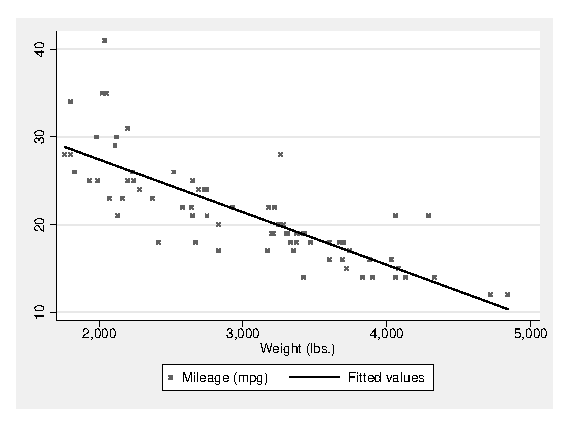
\epsfig{file=output1}
\end{center}
\caption{Scatterplot with simple linear regression line}
\label{fig}
\end{figure}
\end{verbatim}
\end{stverbatim}

\noindent
The graph was generated by running \texttt{output.do}, the
do-file given in section~\ref{sec:output}.  The \texttt{epsfig} package is
described in \citet*{latexcompanion}.

\begin{figure}[h!]
\begin{center}
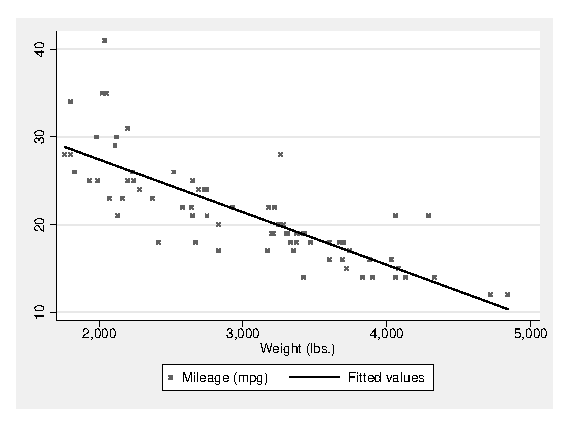
\epsfig{file=output1}
\end{center}
\caption{Scatterplot with simple linear regression line}
\label{fig}
\end{figure}

\subsection{Saved results}

The \texttt{stresults} environment provides a table to describe the saved
results of a Stata command.  It consists of four columns: the first and third
column are for Stata result identifiers (e.g., \stcmd{r(N)}, \stcmd{e(cmd)}),
and the second and fourth columns are for a brief description of the
respective identifier.
%
Each group of results is generated using the \verb+\stresultsgroup+ macro.
%
The following is an example containing a brief description of the results that
\stcmd{regress} saved to \stcmd{e()}:

\begin{stresults}
\stresultsgroup{Scalars} \\
\stcmd{e(N)} & number of observations
&
\stcmd{e(F)} & $\scriptstyle F$ statistic
\\
\stcmd{e(mss)} & model sum of squares
&
\stcmd{e(rmse)} & root mean squared error
\\
\stcmd{e(df\_m)} & model degrees of freedom
&
\stcmd{e(ll\_r)} & log likelihood
\\
\stcmd{e(rss)} & residual sum of squares
&
\stcmd{e(ll\_r0)} & log likelihood, constant-only\\
\stcmd{e(df\_r)} & residual degrees of freedom
&
& \quad model \\
\stcmd{e(r2)} & $\scriptstyle R$-squared
&
\stcmd{e(N\_clust)} & number of clusters
\\
\stresultsgroup{Macros} \\
\stcmd{e(cmd)} & \stcmd{regress}
&
\stcmd{e(wexp)} & weight expression
\\
\stcmd{e(depvar)} & name of dependent variable
&
\stcmd{e(clustvar)} & name of cluster variable
\\
\stcmd{e(model)} & \stcmd{ols} or \stcmd{iv}
&
\stcmd{e(vcetype)} & title used to label Std. Err.
\\
\stcmd{e(wtype)} & weight type
&
\stcmd{e(predict)} & program used to implement
\\
&&&\quad \stcmd{predict}
\\
\stresultsgroup{Matrices} \\
\stcmd{e(b)} & coefficient vector
&
\stcmd{e(V)} & variance--covariance matrix of
\\
&&&\quad the estimators\\
\stresultsgroup{Functions} \\
\stcmd{e(sample)} & marks estimation sample
\\
\end{stresults}

\subsection{Examples and notes}

The following are environments for examples and notes similar to those
given in the Stata reference manuals.  They are generated using the
\texttt{stexample} and \texttt{sttech} environments, respectively.


\begin{stexample}
This is the default alignment for a \stata{} example.
\end{stexample}

\setlength{\stexamplehskip}{0pt}
\begin{stexample}
For this example, \verb+\stexamplehskip+ was set to
\texttt{\the\stexamplehskip}
before beginning.  This sentence is supposed to spill
over to the next line, thus revealing that the first sentence was indented.

This sentence is supposed to show that new paragraphs are automatically
indented (provided that \verb+\parindent+ is nonzero).
\end{stexample}

\begin{sttech}
For this note, \verb+\sttechhskip+ was set to \texttt{\the\sttechhskip}
(the default) before beginning.  This sentence is supposed to spill over to
the next line, thus revealing that the first sentence was indented.

This sentence is supposed to show that new paragraphs are automatically
indented (provided that \verb+\parindent+ is nonzero).
\end{sttech}

\subsection{Special characters}

Table \ref{table:specialch} contains macros that generate some useful
characters in the typewriter (fixed width) font.  The exceptions are
\verb+\stcaret+ and \verb+\sttilde+, which use the currently specified font;
the strictly fixed-width versions are \verb+\caret+ and \verb+\tytilde+,
respectively.

\begin{table}[h!]
\caption{Special characters}
\label{table:specialch}
\begin{center}
\begin{tabular}{ll@{\hspace{.5in}}ll}
\hline
\noalign{\smallskip}
Macro & Result &
Macro & Result \\ 
\noalign{\smallskip}
\hline
\noalign{\smallskip}
\verb+\stbackslash+ & \stbackslash
 &
\verb+\sttilde+ & \sttilde
\\
\verb+\stforslash+ & \stforslash 
&
\verb+\tytilde+ & \tytilde
\\
\verb+\stcaret+ & \stcaret
&
\verb+\lbr+ & \lbr
\\
\verb+\caret+ & \caret
&
\verb+\rbr+ & \rbr
\\
\noalign{\smallskip}
\hline
\end{tabular}
\end{center}
\end{table}


\subsection{Equations and formulas}

In (\ref{eq:Exbar}), $\stbar{x}$ was generated using
\verb+\stbar{x}+.  Here \verb+\stbar+ is equivalent to the \TeX{} macro
\verb+\overline+.

\begin{equation}
E(\stbar{x}) = \mu
\label{eq:Exbar}
\end{equation}

In (\ref{eq:varbetahat}), $\sthat{\beta}$ was generated using
\verb+\sthat{\beta}+.  Here \verb+\sthat+ is equivalent to the \TeX{} macro
\verb+\widehat+.

\begin{equation}
V(\sthat{\beta}) = V\{(X'X)^{-1}X'y\} = (X'X)^{-1}X'V(y)X(X'X)^{-1}
\label{eq:varbetahat}
\end{equation}

\subsection{Other miscellaneous macros and environments}

The following box was created by

\begin{stverbatim}
\begin{verbatim}
\begin{ttbox}
A special framed
box that obeys lines and spaces.
\end{ttbox}
\end{verbatim}
\end{stverbatim}

\begin{ttbox}
A special framed
box that obeys lines and spaces.
\end{ttbox}

\clearpage
The following box was created by

\begin{stverbatim}
\begin{verbatim}
\ttboxWd=2.5in
\ttboxIndent=2em
\begin{ttbox}
Test that the width of the
box is \the\ttboxWd
and is indented \the\ttboxIndent
\end{ttbox}
\end{verbatim}
\end{stverbatim}

\ttboxWd=2.5in
\ttboxIndent=2em
\begin{ttbox}
Test that the width of the
box is \the\ttboxWd
and is indented \the\ttboxIndent
\end{ttbox}

\endinput
